\documentclass[10pt,a4paper]{article}

% Packages
\usepackage[utf8]{inputenc}
\usepackage[spanish, es-tabla]{babel}
\usepackage{caption}
\usepackage{listings}
\usepackage{enumerate}
\usepackage{adjustbox}
\usepackage{enumitem}
\usepackage{boldline}
\usepackage{amssymb, amsmath}
\usepackage[margin=1in]{geometry}
\usepackage{xcolor}
%\usepackage{soul}
\usepackage{enumerate}
\usepackage{hyperref}
\usepackage{graphics, graphicx, float}
\usepackage{booktabs}
%\usepackage[dvipsnames]{xcolor}

% Meta
\title{\textbf{\huge Metaheurísticas: Trabajo Final }
	\\\medskip \Large Algoritmo de la selección clonal (CLONALG)\\ para la optimización de funciones con variables reales \\\medskip}
\author{Pilar Navarro Ramírez - 76592479H \\ pilarnavarro@correo.ugr.es }
\date{ \today }

% Custom
\providecommand{\abs}[1]{\lvert#1\rvert}
\setlength\parindent{0pt}
\definecolor{Light}{gray}{.90}
\newcommand\ddfrac[2]{\frac{\displaystyle #1}{\displaystyle #2}}
\setlength{\parindent}{1.5em} %sangria
\setlength{\parskip}{3mm}

% Displaying code with lstlisting
\lstset { %
	language=C++,
	backgroundcolor=\color{black!5}, % set backgroundcolor
	basicstyle=\small,% basic font setting
}

\usepackage[ruled]{algorithm2e}


\begin{document}	
	
	\maketitle 
	\newpage
	\tableofcontents
	\newpage
	
	
	
	\section{Descripción del algoritmo}
	
	\subsection{El sistema inmunológico}
	
	Hay una serie de características interesantes que presenta el \underline{sistema
	inmunológico humano} y que pueden ser útiles a la hora de desarrollar algoritmos
	basados en su funcionamiento. La inmunidad es una capacidad
	defensiva de un organismo frente a agentes patógenos. Los microorganismos patógenos tiene en su superficie
	antígenos y penetran al organismo pudiendo resultar dañinos para éste.
	
	El sistema inmunológico está constituido por un
	complejo sistema de biomoléculas y células capaces de neutralizar e incluso destruir
	a los agentes infecciosos. Por lo tanto, una de sus primeras funciones será distinguir
	los agentes no propios de los propios y mediante un complejo proceso de
	aprendizaje y memoria lograr neutralizar a los agentes externos.
	
	La respuesta inmunitaria puede ser de dos tipos, \underline{innata o adaptativa}. La respuesta inmunitaria innata actúa con carácter general contra agentes patógenos o infecciosos y su poder de acción no
	mejora con sucesivas infecciones, es decir, se mantiene invariante, lo cual no resulta
	interesante a la hora de desarrollar algoritmos que vayan evolucionando hasta
	llegar a una solución óptima. Pero, la respuesta adaptativa sí que tiene una
	resistencia que mejora tras sucesivas infecciones utilizando para ello una memoria
	inmunológica.
	
		Las células que aparecen en el sistema inmunitario adaptativo son los linfocitos. En concreto aparecen, dos tipos de células principalmente, las \textit{células B y T}.
	Los linfocitos B secretan a su vez, otro tipo de células denominadas \underline{anticuerpos}. Ante la
	presencia de un antígeno, únicamente los linfocitos con anticuerpos que posean la forma
	específica al antígeno, es decir los más afines, serán estimulados para proceder a la eliminación
	del antígeno. Los anticuerpos poseen en su estructura externa una región con una forma
	específica denominada \textit{paratope} que se acopla con su contraparte \textit{epitope} localizada en la
	estructura del antígeno, para reconocer al invasor. Cada linfocito B posee en su superficie
	anticuerpos con el mismo tipo de paratope y los antígenos poseen diferentes tipos de epitopes,
	de manera que un mismo antígeno puede activar varios linfocitos a la vez siendo reconocido por
	éstos.
		
	Los \underline{\textit{Sistemas Inmunológicos Artificiales (SIA)}} tratan de simular el comportamiento del sistema inmunológico humano con la finalidad de resolver problemas computacionales. Los SIA se caracterizan por poseer estructuras híbridas y algoritmos que copian mecanismos inmunológicos. Dichos algoritmos computacionales están basados en principios inmunológicos, como la Teoría de la Selección Clonal.
	
	Las propiedades del Sistema Inmunológico que han despertado
	el interés de científicos, ingenieros, matemáticos y otros investigadores son las siguientes:
	
	\begin{itemize}
		\item \textbf{Unicidad:} Cada individuo posee su propio Sistema Inmunológico, con sus
		características y vulnerabilidades particulares.
		
		\item \textbf{Reconocimiento de cuerpos extraños:} Las moléculas no naturales al cuerpo
		son reconocidas y eliminadas por el Sistema Inmunológico.
		
		\item \textbf{Detección de anomalías:} El Sistema Inmunológico puede detectar y
		reaccionar contra patógenos que nunca antes hayan entrado en contacto con
		el cuerpo.
		
		\item \textbf{Detección distribuida:} Las células del sistema están distribuidas por todo el
		cuerpo sin estar sujetas a ningún control centralizado.
		
		\item \textbf{Detección imperfecta:} No se requiere un reconocimiento absoluto de los
		patógenos, de ahí que el sistema sea flexible.
	\end{itemize}

	Los Algoritmos Genéticos (AG) y los Sistemas Inmunológicos Artificiales poseen
	componentes similares. Sin embargo, se ha comprobado que los SIA presentan grandes
	ventajas sobre los AG. La propiedad más importante de los SIA es la velocidad de convergencia hacia la función objetivo que los convierte en una mejor alternativa frente a los AG.
	
	\subsection{La Teoría de la Selección Clonal}
	
	A continuación, describimos los procesos más destacados de la \underline{Teoría de la selección clonal}:\\
	En primer lugar, la proliferación y diferenciación de las células que han
	sido capaces de reconocer al antígeno. Después, aparece un proceso de
	maduración, mutación somática, en diversos patrones de los anticuerpos, donde se
	generan nuevos cambios genéticos aleatorios que son los encargados de lidiar
	contra el antígeno reconocido. Y, finalmente, aparece un proceso de selección de
	células B, donde, aquellas células con mayor afinidad respecto al antígeno, entrarán
	en un conjunto de células de memoria, y las que presenten menor afinidad serán
	eficientemente eliminadas o modificadas, en su defecto.
	
	En el transcurso de vida de un organismo, éste se puede encontrar
	varias veces con un determinado antígeno. En la respuesta inmune podemos
	distinguir tres tipos de respuestas: \textit{la respuesta primaria, la secundaria}
	\textit{y la reactividad inmunológica cruzada}, las cuales ocurren siguiendo una línea temporal.
	
	En la \underline{primera exposición} el antígeno se encontrará con un bajo número de
	células B con baja afinidad.
	
	El primer paso que realiza el sistema inmunológico adaptativo es reconocer el antígeno o patógeno infeccioso
	que no es propio del organismo. Cualquier molécula no propia del organismo puede
	ser reconocida como un antígeno por el sistema inmunológico adaptativo. Este
	procedimiento es llevado a cabo por las células T que son capaces de reconocer un
	objetivo no propio del organismo.
	
	A continuación, cada patógeno es recordado por un antígeno característico que desencadena una formación de anticuerpos que son	capaces de lidiar con este único antígeno. Los linfocitos B logran identificar los patógenos cuando los anticuerpos de su superficie se unen a determinados antígenos no propios.
	
	Una vez ligado el anticuerpo al antígeno y activado el procedimiento de ataque contra el agente patógeno las células B y T se dividen y se crean millones de copias de ellas, en lo que se denomina respuesta primaria. De todas estas copias	algunas pasan a formar parte de un conjunto de \textit{células de memoria} con un largo periodo de vida. Estas células son las encargadas de recordar cada patógeno
	específico que se hayan encontrado a lo largo de la vida de un ser humano.
	
	Finalmente, gracias a estas células de memoria se consiguen establecer respuestas específicas en sucesivas infecciones para poder eliminar lo más rápidamente posible al patógeno infeccioso. La efectividad de la respuesta inmunológica, por lo tanto, dependerá en gran medida de estas células de memoria
	asociadas desde la primera infección y que son capaces de producir anticuerpos de
	alta afinidad a lo largo de sucesivos encuentros con el antígeno correspondiente.
	
	Después de la respuesta primaria, aparecerá lo que se denomina \underline{respuesta
	secundaria}. Ésta se caracteriza por un periodo de respuesta más corto, una
	velocidad en todo el proceso mayor y una alta concentración de anticuerpos con
	elevada afinidad.
	
	Tras sucesivos encuentros, el sistema inmunológico se va a ir adaptando a las infecciones atacantes y se preparará para futuros ataques de antígenos similares, en lo que se denomina \underline{reactividad inmunológica cruzada.}

	En resumen, la memoria y el aprendizaje inmune es obtenido siguiendo los siguientes pasos:
	\begin{enumerate}
		\item Exposición repetida ante un antígeno
		\item Maduración de la afinidad de las moléculas receptoras		
		\item Disminución del grado de infección crónica
		\item Reactividad inmunológica cruzada
	\end{enumerate}

	Lo que se conoce como \underline{maduración de la respuesta inmune} es debido a que
	los anticuerpos presentes en las sucesivas respuestas por haber pertenecido al
	conjunto de memoria tienen, en general, una mayor afinidad que aquellos que
	participaron en la respuesta primaria. Esta afinidad va aumentando debido a unos
	cambios aleatorios que se van introduciendo en los genes encargados de las
	interacciones entre los anticuerpos y el antígeno. Luego, una vez realizados estos
	cambios, pasarán a formar parte del set de memoria los elementos con mayor
	afinidad.

	Para lograr una rápida maduración de la respuesta inmune se necesitan
	continuas mutaciones de la población, pero la mayoría de estos cambios pueden
	llevar a empeorar los anticuerpos y hacerlos inservibles. Por lo tanto, hay que
	controlar esta mutación, ya que podría darse el caso de que un anticuerpo útil
	mutara y pasara a tener una peor afinidad, lo cual nos conduciría a una mala
	solución. Para solucionar este problema el mecanismo de mutación debe tener en
	cuenta la afinad del anticuerpo, y mutar de forma proporcional a esta. Así, en
	células con una alta afinidad la hipermutación debe mantenerse inactiva o
	prácticamente inactiva. Y, en cambio, en células con una baja afinidad la
	hipermutación debe ser más agresiva y veloz. De este modo nos aseguraremos de
	que el mecanismo converja y llegue a una solución óptima.

	\subsection{El Algoritmo de Selección Clonal (CLONALG)}
	
	El \textbf{Algoritmo de Selección Clonal (ClonalG)} es una implementación computacional
	basada en la Teoría de la Selección Clonal, englobando el proceso de \textit{maduración de
	la respuesta inmune, o maduración de afinidad}. 

	Los principios inmunológicos tomados en cuenta en este algoritmo son:	
	\begin{itemize}
		\item El mantenimiento de células de memoria.
		\item Selección y clonación de los individuos más estimulados.
		\item Muerte de las células no estimuladas.
		\item Maduración de Afinidad y selección de los clones con mayor afinidad.
		\item Generación y mantenimiento de la diversidad.
		\item Hipermutación proporcional a la afinidad celular.
	\end{itemize}	
	A grandes rasgos, el funcionamiento del algoritmo es el siguiente: dada una
	población de anticuerpos (soluciones), donde cada uno de ellos tiene asociado un valor de afinidad
	(correspondiente al valor de la función objetivo), se seleccionan para ser clonados aquellos
	individuos con mejor afinidad.
	
	Los anticuerpos seleccionados serán clonados proporcionalmente a su afinidad generando un
	repertorio de clones. Cada uno de los clones es hipermutado (mutación a gran escala) de forma
	inversamente proporcional a su afinidad, para luego seleccionar los mejores individuos entre la
	población de clones y la población de anticuerpos. Por último se reemplazan los individuos de
	menor afinidad por individuos generados aleatoriamente.
	
	El algoritmo ClonalG considera una colección de vectores, integrada por los anticuerpos \textbf{Ab}, que nosotros llamaremos población (population). 
	
	Los pasos del algoritmo son los siguientes:	
	\begin{enumerate}
		\item  Generar aleatoriamente una población de anticuerpos \textit{Ab}, con tamaño N. Para nuestra implementación la población será de tamaño 50.
		
		\item Calcular la afinidad \textit{f} de cada anticuerpo de \textit{Ab}. La afinidad está descrita en
		términos de una función de fitness \textit{f}.
		
		\item Seleccionar los $ n $ anticuerpos $ Ab_j $ , $ (j= 1,..., n) $, con la afinidad más alta (conjunto $ Ab_n $).		
		
		\item Clonar los anticuerpos pertenecientes al conjunto de anticuerpos de alta afinidad. Esta clonación puede realizarse de forma proporcional a su afinidad o se puede clonar a todos los
		anticuerpos en la misma medida. Se formará el conjunto de clones $C$.
		
		\item Los elementos clonados se mutan para aumentar la diversidad. El proceso de
		mutación debe ser inversamente proporcional a la afinidad, es decir, los
		elementos con mayor afinidad deben mutar menos, y los elementos con peor
		afinidad mutan más para que la población llegue a converger. $C^{*}$ es el conjunto
		de clones mutados.
		
		\item Calcular la afinidad $ f^* $ de los clones mutados $ C^* $.
		
		\item Seleccionar los $ n $ mejores anticuerpos $ Ab_k $, $k=(1,..., n)$, para que formen parte del set de memoria,$Ab_m$
		
		\item Sustituir los $ d $ anticuerpos de menor afinidad por nuevos anticuerpos (conjunto $ Ab_d $)
	\end{enumerate}
	\begin{figure}[H]
		\centering
		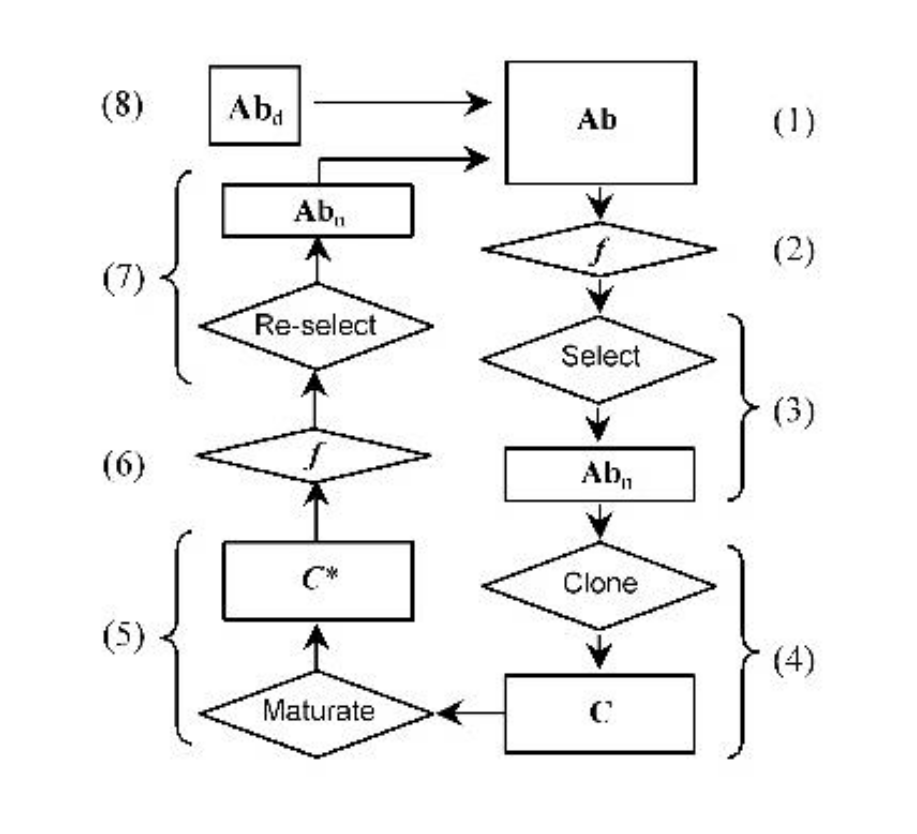
\includegraphics[width=0.8\linewidth]{img/diagrama}
		\caption{Diagrama de flujo del Algoritmo ClonalG}
		\label{fig:diagrama}
	\end{figure}
	
	Usaremos el algortimo para buscar el mínimo de 30 funciones de variables reales, en espacios de 10 y 30 dimensiones. Cada una de las variables toma un valor real en el intervalo $ [-100,100] $.
\newpage
	\section{Pseudo-códigos}
	
	\subsection{Representación de la soluciones}
	
	Una solución vendrá dada como un vector de valores reales en el intervalo $ [-100,100] $, de tamaño igual a la dimensión del espacio en el que esté definida la función que se busca optimizar.
	Asociado a este vector tendremos dos parámetros adicionales: el \textit{fitness} de la solución determinada por el vector y un booleano que servirá para indicar si la solución ha sido o no evaluada (se ha calculado su fitness), de manera que se evite evaluar varias veces la misma solución. Así, la estructura de una solución (anticuerpo) será la siguiente:
	
	\begin{lstlisting}
	struct Antibody {
		vector<double> elements;
		double fitness;
		bool evaluated;
	};
	\end{lstlisting}
	
	Por otra parte, se representa una población como un vector de anticuerpos, con un tamaño igual al de la población, esto es, el número de anticuerpos que tiene esa población. Junto al vector de soluciones se guarda también el fitness del anticuerpo de mayor afinidad de la población y la posición en el vector del mismo:
	
		\begin{lstlisting}
	struct population {
		vector<Antibody> solutions;
		double best_fitness;	//Fitness de la mejor solucion
		int best_sol;		//Posicion de la mejor solucion
	};
	\end{lstlisting}
	
	
	\subsection{Evaluación de una población}
	Con el objetivo de evaluar una población de soluciones (anticuerpos) implementamos la función \lstinline|evaluatePopulation|, que se encarga de calcular el fitness de todas las soluciones de la población que aún no han sido evaluadas y determinar la posición y el fitness de la mejor solución contenida en la población:
	
		\begin{algorithm}[H]
		\DontPrintSemicolon
		\caption{\sc evaluatePopulation}
		\KwIn{población \textit{pop} a ser evaluda, número de evaluaciones \textit{evaluations}}
		\KwOut{población \textit{pop} evaluada}
		\Begin{
			$ best\_pos $ $ \leftarrow $ $ pop.best\_sol $ \\
			$ best\_fit $ $ \leftarrow $ $ pop.best\_fitness $
			
			\For { $ sol $ \textbf{in} $ pop.solutions $ }{
				\If{sol \textbf{is not} evaluated \textbf{and} evaluations$<10000dim$}{\tcp*{dim es la dimensión del espacio}
				evaluations ++\\
				sol.fitness $ \leftarrow $ $\operatorname{cec17\_fitness}(sol, matrix)$\\
				sol.evaluated $\leftarrow$ true \\
				\If{$ best\_fit $ $ > $ sol.fitness}
				{$ best\_fit $ $\leftarrow$ sol.fitness \\
				$ best\_pos $ $\leftarrow$ $ index\_of(sol) $}
				}					
				}
			
			$ pop.best\_fitness $ $\leftarrow$ $ best\_fit $ \\
			$ pop.best\_sol $ $\leftarrow$ $ best\_pos $ \\
			\Return pop
		}
	\end{algorithm}
	
	Notamos que tras cada llamada a la función \textit{fitness} para una solución, se aumenta el número de evaluaciones de dicha función (\textit{evaluations})
	
	\subsection{Generación de una población aleatoria}
	Para generar las soluciones aleatorias usamos la función \lstinline|randomSolution|:
	
	\begin{algorithm}[H]
		\DontPrintSemicolon
		\caption{\sc randomSolution}
		\KwOut{solución aleatoria}
		\Begin{
			$sol \leftarrow [0,0,...^{dim)},0]$\tcp*{Partimos de una solución con todos los valores nulos} 
		
		\ForEach{ $ i \in \{0,...,dim-1\}$ }{  
				$sol[i] \leftarrow$ valor real aleatorio en el intervalo $ [-100,100] $\\	
		}
		sol.evaluated $\leftarrow$ false\\
		\Return sol
		}
	\end{algorithm}

La función \lstinline|randomPopulation| se encarga de generar la población inicial aleatoriamente haciendo uso de la función anterior como se muestra a continuación:

	\begin{algorithm}[H]
	\caption{\sc randomPopulation}
	\KwIn{tamaño de la población $ size\_pop $, número de evaluaciones de la función objetivo $ evaluations $}
	\KwOut{población de anticuerpos correctamente evaluada}
	\Begin{
		\For{i \textbf{in} $[0,size\_pop)$}{
			sol $\leftarrow$ $\operatorname{randomSolution}()$\\
			pop.solutions $\leftarrow$ pop.solutions $\cup$ $ \{sol\} $
		}
		$ pop.best\_sol $ $\leftarrow$ -1\\
		$ pop.best\_fitness $ $\leftarrow \infty$ \\
		$\operatorname{evaluatePopulation}(pop,evaluations)$\\
		\Return pop
	}
\end{algorithm}

\subsection{Selección de los anticuerpos más afines}

El proceso de selección consiste en escoger los anticuerpos de la población que tienen mayor afinidad (menor valor de fitness en nuestro problema). Nos quedaremos con el $ 30\% $ de los mejores anticuerpos de la población, dando lugar a una nueva población de anticuerpos de menor tamaño. Para ello, se ordenan los anticuerpos de menor a mayor fitness y se seleccionan los $size\_pop\times0.3$ primeros, que pasan a formar parte de otra población. El pseudo-código de este operador se muestra a continuación: 

\begin{algorithm}[H]
	\DontPrintSemicolon
	\caption{{\sc selection} }
	\KwIn{Población \textit{old\_pop}, proporción de las mejores soluciones a seleccionar \textit{perc\_sel}}
	\KwOut{Nueva población con las mejores soluciones $ new\_pop $}
	\Begin{
		$num\_sel \leftarrow perc\_sel*old\_pop.solutions.size()$\\
		$new\_pop.solutions\leftarrow [0,..^{num\_sel)}.,0]$\\
		sort $old\_pop.solutions$ de menor a mayor fitness\\

		\ForEach{$ i \in \{0,...,num\_sel-1\} $}{
			$new\_pop.solutions[i] \leftarrow$ $ old\_pop.solutions[i] $
		}
		$new\_pop.best\_fitness\leftarrow new\_pop.solutions[0].fitness $\\
		$new\_pop.best\_sol\leftarrow 0$\\
		\Return $ new\_pop $
	}
\end{algorithm}

\subsection{Clonación de anticuerpos}

Creamos una población de clones, $C$, a partir de la población seleccionada con los anticuerpos de mayor afinidad. Esta población de clones estará formada por el 50\% de los mejores anticuerpos de $new\_pop$. Como en el operador de  selección las soluciones de $new\_pop$ se seleccionan de forma ordenada, de menor a mayor fitness, bastará asignar a $C$ los 50\% primeros anticuerpos de $new\_pop$. De esta forma se duplican los anticuerpos más afines. 

\begin{algorithm}[H]
	\DontPrintSemicolon
	\caption{{\sc clone} }
	\KwIn{Población \textit{new\_pop}, proporción de las mejores soluciones a clonar \textit{perc\_clone}}
	\KwOut{Población de clones $C$}
	\Begin{
		$num\_clones \leftarrow perc\_clone*new\_pop.solutions.size()$\\
		$C.solutions\leftarrow [0,..^{num\_clones)}.,0]$\\
	
		\ForEach{$ i \in \{0,...,num\_clones-1\} $}{
			$C.solutions[i] \leftarrow$ $ new\_pop.solutions[i] $
		}
		$C.best\_fitness\leftarrow C.solutions[0].fitness $\\
		$C.best\_sol\leftarrow 0$\\
		\Return $ C $
	}
\end{algorithm}

\subsection{Mutación de los clones}

Con este operador se mutan las soluciones de la población $C$ de manera inversamente proporcional a su afinidad. En concreto, cada solución de la población pasada como parámetro se muta tantas veces como indica su posición en el vector de soluciones, esto es, la solución de la posición 0, que será la más afín, no se muta nunca, la de la posición 1 se mutará una única vez, y así sucesivamente, de modo que la última solución, la menos afín, es la que más veces muta. Para la mutación lo que se hace es elegir una posición aleatoria de la solución, correspondiente a una variable, y se le cambia el valor por otro aleatorio del intervalo $[-100,100]$. 

\begin{algorithm}[H]
	\DontPrintSemicolon
	\caption{{\sc mutation} }
	\KwIn{Población \textit{C} a mutar}
	\Begin{
		\ForEach{$ i \in \{0,...,C.solutions.size()-1\} $}{
			\ForEach{$ j \in \{0,...,i-1\} $}{
			pos $\leftarrow$  número aleatorio entre 0 y $ dim $ \tcp*{dim es el tamaño de una solución}
			C.solutions[i].elements[pos] $\gets$ valor real aleatorio en el intervalo $ [-100,100] $\\
			C.solutions[i].elements[pos].evaluated $\gets false$
		}
		}
	}
\end{algorithm}

\subsection{Operador de reemplazamiento}

Para reemplazar los peores anticuerpos de una población por todos los de otra de menor tamaño, implementamos el operador de reemplazamiento. Este se encarga de introducir las soluciones de la última en las posiciones de las peores soluciones de la primera, que serán las últimas posiciones del vector cuando los anticuerpos estén ordenados de mayor a menor afinidad.  Así nos aseguramos que las mejores soluciones (los anticuerpos más afines) siempre se mantienen en la población. 

\begin{algorithm}[H]
	\DontPrintSemicolon
	\caption{{\sc replace} }
	\KwIn{Dos poblaciones de soluciones $ new\_pop $ y $old\_pop$}
	\KwOut{Población $old\_pop$ con las soluciones de $ new\_pop $}
	\Begin{
		
		size $\gets old\_pop.solutions.size()$\\
		sort $old\_pop.solutions$ de menor a mayor fitness\\
		
		\ForEach{i $\in \{0,...,new\_pop.solutions.size()-1\}$ }{
		
		$old\_pop.solutions[size-1-i] \gets new\_pop.solutions[i]$\\
	
		}
		sort $old\_pop.solutions$ de menor a mayor fitness\\
		
		$old\_pop.best\_fitness\leftarrow old\_pop.solutions[0].fitness $\\
		$old\_pop.best\_sol\leftarrow 0$\\
		
		
		\Return old\_pop
	}
\end{algorithm}

\subsection{Reemplazamiento de las peores soluciones}

El último paso de nuestro algoritmo consiste en eliminar los anticuerpos menos afines de la población, mediante la sustitución de los mismos por anticuerpos totalmente nuevos. Lo que haremos será generar nuevas soluciones aleatorias, que reemplazarán al 10\% de los peores anticuerpos. Para ello, haremos uso de la siguiente función:

\begin{algorithm}[H]
	\DontPrintSemicolon
	\caption{{\sc replaceWorst} }
	\KwIn{Población de soluciones $pop$,  proporción de las peores soluciones a reemplazar \textit{perc\_worst}}
	\KwOut{Población $pop$ con las peores soluciones reemplazadas}
	\Begin{
		
		size $\gets pop.solutions.size()$\\
		num\_replace $\gets size\times perc\_worst$
		
		\ForEach{i $\in \{0,...,num\_replace-1\}$}{	
			$pop.solutions[size-1-i] \gets randomSolution()$\\		
		}
		
		sort $pop.solutions$ de menor a mayor fitness\\
		
		$pop.best\_fitness \leftarrow pop.solutions[0].fitness $\\
		$pop.best\_sol\leftarrow 0$\\
		
		
		\Return pop
	}
\end{algorithm}

\subsection{Pseudo-código principal}

Podemos ya presentar el pseudo-código principal de nuestro algoritmo, que hace uso de los operadores ya descritos: 

\begin{algorithm}[H]
	\DontPrintSemicolon
	\caption{{\sc CLONALG}}
	\KwOut{Anticuerpo de mayor afinidad de la población obtenida tras varias iteraciones}
	\Begin{
		evaluations $\leftarrow$ 0\\
		size\_pop $\leftarrow$ 50 \\
		perc\_sel $\leftarrow$ 0.3 \tcp*{Proporción de mejores soluciones a seleccionar}
		perc\_clone $\leftarrow$ 0.5 \tcp*{Proporción de anticuerpos de alta afinidad a clonar}
		perc\_worst $\leftarrow$ 0.1 \tcp*{Proporción de peores soluciones a reemplazar}
		old\_pop $\leftarrow$ randomPopulation(size\_pop,evaluations) \tcp*{Partimos de una población\\ aleatoria}
		\While{evaluations $< 10000 \times dim$}{
		new\_pop $\leftarrow$ selection(old\_pop, perc\_sel)\\
		C $\leftarrow$ clone(new\_pop, perc\_clone)\\
		mutation(C)\\
		\tcp{Evaluamos las soluciones de la población de clones mutados}
		C $\leftarrow$ evaluatePopulation(C,evaluations)\\
		\tcp{Introducimos los clones mutados en new\_pop}
		new\_pop $\gets$ replace(new\_pop,C) \\
		\tcp{Introducimos los anticuerpos de new\_pop en old\_pop}
		old\_pop $\gets$ replace(old\_pop,new\_pop) \\
		\tcp{Reemplazamos las peores soluciones por nuevas aleatorias}
		old\_pop $\gets$ replaceWorst(old\_pop,perc\_worst) \\
		\tcp{Evaluamos las soluciones de la población old\_pop}
		old\_pop $\leftarrow$ evaluatePopulation(old\_pop,evaluations)\\
		}
		\Return old\_pop.best\_sol
	}
\end{algorithm}

\newpage
	
\section{Experimentos y análisis de resultados}

	Presentaremos aquí una análisis de los resultados proporcionados por nuestro algoritmo y realizaremos una comparativa con otras metaheurísticas que participaron en la competición CEC2017. En concreto, compareremos con DE, PSO, AEO y SSA, que son los recomendados en clase.  
	
 	Mostramos en las siguientes tablas los resultados obtenidos para cada algoritmo. Se presenta el
	error medio en 10 ejecuciones con distintas semillas para cada una de las 30 funciones. Para la ejecución i-ésima se utiliza la semilla $i-1$, de modo que la primera ejecución usa como semilla el 0, la segunda el 1, y así sucesivamente.	

	\subsection{Resultados obtenidos en dimensión 10 para el 100\% de las evaluaciones}
	
	\begin{table}[H]
	\begin{center}	
	\begin{tabular}{llllll}
		\toprule
		{} &         AEO &          DE &       CLONALG &         PSO &         SSA \\
		\midrule
		F01  &  5.1338e+06 &  0.0000e+00 &  5.6263e+08 &  5.2551e+07 &  3.7658e+03 \\
		F02  &  1.0000e+00 &  0.0000e+00 &  1.0783e+07 &  1.0000e+00 &  1.0000e+00 \\
		F03  &  3.5753e+02 &  0.0000e+00 &  4.0079e+03 &  1.9889e+03 &  1.0000e-10 \\
		F04  &  1.4145e+01 &  1.1050e-04 &  4.8146e+01 &  4.6843e+01 &  4.1722e+00 \\
		F05  &  3.8755e+01 &  1.1508e+02 &  3.3791e+01 &  3.2120e+01 &  4.8404e+01 \\
		F06  &  2.6171e+01 &  3.4597e+01 &  1.4146e+01 &  1.0010e+01 &  2.6321e+01 \\
		F07  &  6.7525e+01 &  3.8481e+01 &  9.0437e+01 &  4.2752e+01 &  6.1980e+01 \\
		F08  &  2.8081e+01 &  2.9829e+01 &  3.7601e+01 &  2.2032e+01 &  3.8487e+01 \\
		F09  &  2.2069e+02 &  1.9379e+02 &  1.8754e+02 &  5.6865e+01 &  2.4393e+02 \\
		F10  &  1.1717e+03 &  3.5968e+02 &  8.0714e+02 &  1.0769e+03 &  1.0857e+03 \\
		F11  &  9.7039e+01 &  1.9419e-02 &  2.8942e+03 &  3.8427e+01 &  9.5287e+01 \\
		F12  &  2.5246e+05 &  4.9311e+00 &  2.8818e+07 &  2.5169e+06 &  2.3135e+04 \\
		F13  &  7.7879e+02 &  5.9881e+00 &  1.7461e+07 &  8.4086e+03 &  8.1014e+03 \\
		F14  &  7.4524e+01 &  5.2398e-02 &  2.5060e+05 &  9.9926e+01 &  1.1810e+02 \\
		F15  &  2.0449e+02 &  6.0603e-02 &  2.1689e+06 &  2.0658e+03 &  5.2435e+02 \\
		F16  &  1.8041e+02 &  4.5606e+02 &  2.6339e+02 &  1.4146e+02 &  1.8839e+02 \\
		F17  &  8.9686e+01 &  2.3505e+01 &  1.3200e+02 &  6.4972e+01 &  9.7691e+01 \\
		F18  &  1.9260e+03 &  3.6300e-02 &  4.0082e+06 &  1.4840e+04 &  1.3604e+04 \\
		F19  &  6.4182e+01 &  5.1923e-03 &  1.6991e+06 &  3.2196e+03 &  1.2460e+02 \\
		F20  &  1.2838e+02 &  3.8369e+02 &  1.7590e+02 &  8.4439e+01 &  1.0577e+02 \\
		F21  &  1.7694e+02 &  1.8889e+02 &  2.1136e+02 &  1.3195e+02 &  1.0439e+02 \\
		F22  &  1.1475e+02 &  1.0048e+02 &  1.5235e+02 &  7.7404e+01 &  1.0909e+02 \\
		F23  &  3.4278e+02 &  8.0975e+02 &  3.4365e+02 &  3.3040e+02 &  3.4870e+02 \\
		F24  &  3.4600e+02 &  1.0000e+02 &  3.4709e+02 &  1.8104e+02 &  2.5966e+02 \\
		F25  &  4.3480e+02 &  4.0401e+02 &  4.6033e+02 &  4.4781e+02 &  4.3796e+02 \\
		F26  &  5.0474e+02 &  2.7059e+02 &  7.0964e+02 &  3.7293e+02 &  3.9041e+02 \\
		F27  &  4.1972e+02 &  3.8973e+02 &  4.2152e+02 &  4.1342e+02 &  4.1169e+02 \\
		F28  &  5.4687e+02 &  3.5173e+02 &  5.0192e+02 &  4.6976e+02 &  4.3183e+02 \\
		F29  &  3.7517e+02 &  2.3755e+02 &  3.1311e+02 &  3.1929e+02 &  3.6763e+02 \\
		F30  &  2.4709e+06 &  8.0512e+04 &  9.4311e+05 &  6.3525e+05 &  1.4690e+06 \\
		Best &           0 &          21 &           0 &           8 &           1 \\
		\bottomrule
\end{tabular}
\caption{}
\end{center}
\end{table}

\begin{table}[H]
\begin{center}
	\begin{tabular}{lllll}
		
		\toprule
		{} &         AEO &       CLONALG &         PSO &         SSA \\
		\midrule
		F01  &  5.1338e+06 &  5.6263e+08 &  5.2551e+07 &  3.7658e+03 \\
		F02  &  1.0000e+00 &  1.0783e+07 &  1.0000e+00 &  1.0000e+00 \\
		F03  &  3.5753e+02 &  4.0079e+03 &  1.9889e+03 &  1.0000e-10 \\
		F04  &  1.4145e+01 &  4.8146e+01 &  4.6843e+01 &  4.1722e+00 \\
		F05  &  3.8755e+01 &  3.3791e+01 &  3.2120e+01 &  4.8404e+01 \\
		F06  &  2.6171e+01 &  1.4146e+01 &  1.0010e+01 &  2.6321e+01 \\
		F07  &  6.7525e+01 &  9.0437e+01 &  4.2752e+01 &  6.1980e+01 \\
		F08  &  2.8081e+01 &  3.7601e+01 &  2.2032e+01 &  3.8487e+01 \\
		F09  &  2.2069e+02 &  1.8754e+02 &  5.6865e+01 &  2.4393e+02 \\
		F10  &  1.1717e+03 &  8.0714e+02 &  1.0769e+03 &  1.0857e+03 \\
		F11  &  9.7039e+01 &  2.8942e+03 &  3.8427e+01 &  9.5287e+01 \\
		F12  &  2.5246e+05 &  2.8818e+07 &  2.5169e+06 &  2.3135e+04 \\
		F13  &  7.7879e+02 &  1.7461e+07 &  8.4086e+03 &  8.1014e+03 \\
		F14  &  7.4524e+01 &  2.5060e+05 &  9.9926e+01 &  1.1810e+02 \\
		F15  &  2.0449e+02 &  2.1689e+06 &  2.0658e+03 &  5.2435e+02 \\
		F16  &  1.8041e+02 &  2.6339e+02 &  1.4146e+02 &  1.8839e+02 \\
		F17  &  8.9686e+01 &  1.3200e+02 &  6.4972e+01 &  9.7691e+01 \\
		F18  &  1.9260e+03 &  4.0082e+06 &  1.4840e+04 &  1.3604e+04 \\
		F19  &  6.4182e+01 &  1.6991e+06 &  3.2196e+03 &  1.2460e+02 \\
		F20  &  1.2838e+02 &  1.7590e+02 &  8.4439e+01 &  1.0577e+02 \\
		F21  &  1.7694e+02 &  2.1136e+02 &  1.3195e+02 &  1.0439e+02 \\
		F22  &  1.1475e+02 &  1.5235e+02 &  7.7404e+01 &  1.0909e+02 \\
		F23  &  3.4278e+02 &  3.4365e+02 &  3.3040e+02 &  3.4870e+02 \\
		F24  &  3.4600e+02 &  3.4709e+02 &  1.8104e+02 &  2.5966e+02 \\
		F25  &  4.3480e+02 &  4.6033e+02 &  4.4781e+02 &  4.3796e+02 \\
		F26  &  5.0474e+02 &  7.0964e+02 &  3.7293e+02 &  3.9041e+02 \\
		F27  &  4.1972e+02 &  4.2152e+02 &  4.1342e+02 &  4.1169e+02 \\
		F28  &  5.4687e+02 &  5.0192e+02 &  4.6976e+02 &  4.3183e+02 \\
		F29  &  3.7517e+02 &  3.1311e+02 &  3.1929e+02 &  3.6763e+02 \\
		F30  &  2.4709e+06 &  9.4311e+05 &  6.3525e+05 &  1.4690e+06 \\
		Best &           6 &           2 &          14 &           7 \\

		\bottomrule

	\end{tabular}
		\caption{}
\end{center}	
\end{table}
	\subsection{Resultado obtenidos en dimensión 30 para el 100\% de las evaluaciones}
	\begin{table}[H]
	\begin{center}
	\begin{tabular}{llllll}
		
		\toprule
		{} &         AEO &          DE &       CLONALG &         PSO &         SSA \\
		\midrule
		F01  &  1.7816e+08 &  4.9095e+04 &  2.2724e+09 &  4.1750e+09 &  3.7651e+03 \\
		F02  &  1.0000e+00 &  1.3086e+19 &  2.5513e+26 &  1.0000e+00 &  1.0000e+00 \\
		F03  &  2.9892e+04 &  3.4811e+03 &  2.4412e+04 &  5.4534e+04 &  2.4157e-05 \\
		F04  &  2.0182e+02 &  8.4304e+01 &  2.7245e+02 &  1.1832e+03 &  8.3882e+01 \\
		F05  &  2.4961e+02 &  2.0150e+02 &  1.4907e+02 &  2.1704e+02 &  2.6491e+02 \\
		F06  &  6.8942e+01 &  6.3203e+00 &  1.5992e+01 &  3.6939e+01 &  6.3838e+01 \\
		F07  &  5.2907e+02 &  2.3342e+02 &  3.6553e+02 &  3.5958e+02 &  4.6089e+02 \\
		F08  &  1.8937e+02 &  1.8937e+02 &  1.5267e+02 &  1.7452e+02 &  2.2054e+02 \\
		F09  &  5.9186e+03 &  6.5297e+01 &  1.9454e+03 &  2.8418e+03 &  6.2120e+03 \\
		F10  &  6.0424e+03 &  3.7636e+03 &  4.1400e+03 &  6.9381e+03 &  4.8435e+03 \\
		F11  &  3.9801e+02 &  7.9583e+01 &  2.4914e+03 &  1.2071e+03 &  1.5373e+02 \\
		F12  &  8.5847e+07 &  3.2577e+05 &  2.3205e+08 &  3.5857e+08 &  2.5285e+06 \\
		F13  &  1.8804e+06 &  1.5361e+02 &  3.2311e+08 &  4.5076e+07 &  1.9260e+05 \\
		F14  &  1.7969e+04 &  7.1002e+01 &  2.6433e+06 &  3.0587e+05 &  3.2865e+03 \\
		F15  &  6.1639e+04 &  6.2557e+01 &  1.7529e+08 &  2.7371e+05 &  8.8523e+04 \\
		F16  &  2.0078e+03 &  1.3192e+03 &  1.4822e+03 &  1.5683e+03 &  1.6580e+03 \\
		F17  &  8.2240e+02 &  4.8088e+02 &  5.8395e+02 &  4.7255e+02 &  8.4715e+02 \\
		F18  &  3.1096e+05 &  6.1222e+01 &  6.0420e+06 &  2.1704e+06 &  8.8546e+04 \\
		F19  &  1.8883e+06 &  3.5723e+01 &  1.9816e+08 &  1.2602e+06 &  1.5097e+05 \\
		F20  &  7.2080e+02 &  2.7511e+02 &  6.7691e+02 &  4.6215e+02 &  6.4505e+02 \\
		F21  &  4.4776e+02 &  3.2549e+02 &  3.6732e+02 &  4.1129e+02 &  4.5024e+02 \\
		F22  &  1.9871e+03 &  1.0022e+02 &  4.2837e+03 &  1.0266e+03 &  4.1962e+03 \\
		F23  &  8.4099e+02 &  5.3461e+02 &  5.3548e+02 &  6.4043e+02 &  8.3651e+02 \\
		F24  &  8.7878e+02 &  6.0590e+02 &  6.7249e+02 &  7.0951e+02 &  9.2638e+02 \\
		F25  &  5.0551e+02 &  3.8703e+02 &  5.3004e+02 &  6.8638e+02 &  4.1758e+02 \\
		F26  &  4.5290e+03 &  4.0377e+02 &  2.7231e+03 &  3.3694e+03 &  5.5217e+03 \\
		F27  &  8.1268e+02 &  4.9252e+02 &  5.7747e+02 &  8.0681e+02 &  6.5502e+02 \\
		F28  &  5.5468e+02 &  3.9427e+02 &  5.8566e+02 &  1.1050e+03 &  4.8961e+02 \\
		F29  &  2.0881e+03 &  1.0251e+03 &  9.9714e+02 &  1.4091e+03 &  1.9343e+03 \\
		F30  &  9.8387e+06 &  3.6566e+03 &  4.4247e+07 &  1.3586e+07 &  2.3082e+06 \\
		Best &           0 &          22 &           3 &           1 &           3 \\
		\bottomrule
	\end{tabular}
	\caption{}
\end{center}
\end{table}

\begin{table}[H]
\begin{center}
\begin{tabular}{lllll}
	\toprule
	{} &         AEO &       CLONALG &         PSO &         SSA \\
	\midrule
	F01  &  1.7816e+08 &  2.2724e+09 &  4.1750e+09 &  3.7651e+03 \\
	F02  &  1.0000e+00 &  2.5513e+26 &  1.0000e+00 &  1.0000e+00 \\
	F03  &  2.9892e+04 &  2.4412e+04 &  5.4534e+04 &  2.4157e-05 \\
	F04  &  2.0182e+02 &  2.7245e+02 &  1.1832e+03 &  8.3882e+01 \\
	F05  &  2.4961e+02 &  1.4907e+02 &  2.1704e+02 &  2.6491e+02 \\
	F06  &  6.8942e+01 &  1.5992e+01 &  3.6939e+01 &  6.3838e+01 \\
	F07  &  5.2907e+02 &  3.6553e+02 &  3.5958e+02 &  4.6089e+02 \\
	F08  &  1.8937e+02 &  1.5267e+02 &  1.7452e+02 &  2.2054e+02 \\
	F09  &  5.9186e+03 &  1.9454e+03 &  2.8418e+03 &  6.2120e+03 \\
	F10  &  6.0424e+03 &  4.1400e+03 &  6.9381e+03 &  4.8435e+03 \\
	F11  &  3.9801e+02 &  2.4914e+03 &  1.2071e+03 &  1.5373e+02 \\
	F12  &  8.5847e+07 &  2.3205e+08 &  3.5857e+08 &  2.5285e+06 \\
	F13  &  1.8804e+06 &  3.2311e+08 &  4.5076e+07 &  1.9260e+05 \\
	F14  &  1.7969e+04 &  2.6433e+06 &  3.0587e+05 &  3.2865e+03 \\
	F15  &  6.1639e+04 &  1.7529e+08 &  2.7371e+05 &  8.8523e+04 \\
	F16  &  2.0078e+03 &  1.4822e+03 &  1.5683e+03 &  1.6580e+03 \\
	F17  &  8.2240e+02 &  5.8395e+02 &  4.7255e+02 &  8.4715e+02 \\
	F18  &  3.1096e+05 &  6.0420e+06 &  2.1704e+06 &  8.8546e+04 \\
	F19  &  1.8883e+06 &  1.9816e+08 &  1.2602e+06 &  1.5097e+05 \\
	F20  &  7.2080e+02 &  6.7691e+02 &  4.6215e+02 &  6.4505e+02 \\
	F21  &  4.4776e+02 &  3.6732e+02 &  4.1129e+02 &  4.5024e+02 \\
	F22  &  1.9871e+03 &  4.2837e+03 &  1.0266e+03 &  4.1962e+03 \\
	F23  &  8.4099e+02 &  5.3548e+02 &  6.4043e+02 &  8.3651e+02 \\
	F24  &  8.7878e+02 &  6.7249e+02 &  7.0951e+02 &  9.2638e+02 \\
	F25  &  5.0551e+02 &  5.3004e+02 &  6.8638e+02 &  4.1758e+02 \\
	F26  &  4.5290e+03 &  2.7231e+03 &  3.3694e+03 &  5.5217e+03 \\
	F27  &  8.1268e+02 &  5.7747e+02 &  8.0681e+02 &  6.5502e+02 \\
	F28  &  5.5468e+02 &  5.8566e+02 &  1.1050e+03 &  4.8961e+02 \\
	F29  &  2.0881e+03 &  9.9714e+02 &  1.4091e+03 &  1.9343e+03 \\
	F30  &  9.8387e+06 &  4.4247e+07 &  1.3586e+07 &  2.3082e+06 \\
	Best &           1 &          12 &           4 &          12 \\
	\bottomrule
\end{tabular}
	\caption{}
\end{center}
\end{table}
				
\newpage

	\subsection{ Análisis de los resultados }
	
	En las tablas anteriores podemos ver que nuestro algoritmo presenta errores similares en la mayoría de los casos que los algoritmos de referencia, consiguiendo superar a algunos de ellos para algunas funciones. 
	
	En \underline{dimensión 10}, el algoritmo de DE (\textit{Differential Evolution}) supera al nuestro en casi todas las funciones. No obstante, para las funciones 4, 5, 6 y 9, CLONALG  ofrece un error menor que DE, aunque no consigue superar los errores de los otros algoritmos en estas funciones. 
	
	En la Tabla 2 no se tiene en cuenta DE, que es el mejor de los algoritmos de referencia, y nos damos cuenta entonces de que nuestro algoritmo obtiene el mejor resultado en comparación con PSO, AEO y SSA en 2 de las funciones a optimizar. 
	
	En \underline{dimensión 30} la situación cambia ligeramente, pues CLONALG consigue superar a todos los algoritmos de referencia en 3 de las 30 funciones. Además, obtiene un mejor resulado que PSO, AEO y SSA en 12 funciones, superando así a PSO y AEO con diferencia. 
	Así, podríamos decir que nuestro algoritmo presenta mejores resultados en dimensiones mayores. 
	
	No obstante, para algunas funciones el error ofrecido por CLONALG es muy alto en comparación con los otros algoritmos, como es el caso de la función 2 en dimensión 30, donde el error es del orden de $10^{26}$, o las funciones 1 y 2 en dimensión 10, con errores del orden de $10^8$ y $10^7$, respectivamente. 
	
	En el algoritmo CLONALG, la exploración se lleva a cabo gracias a la hipermutación proporcional a la afinidad celular, mediante la cual las soluciones peores son mutadas en gran medida, favoreciendo así la diversidad y una búsqueda amplia por el espacio de soluciones. Además, el hecho de eliminar las soluciones peores y sustituirlas por otras totalmente aleatorias favorece aún más la exploración, evitando así que el algoritmo quede estancando en óptimos locales. 
	
	Por otra parte, el mantenimiento de células de memoria y la clonación de los anticuerpos más afines favorece la convergencia, permitiendo al algoritmo centrar la búsqueda en zonas del espacio prometedoras. 
	
	Los errores relativamente altos de nuestro algoritmo en algunos casos nos hacen pensar que puede haber un problema de convergencia (que nuestro algoritmo no llegue a converger) o/y exploración (esta no sea suficiente). Sin embargo, a priori sin más experimentos no podemos saber qué parte habría que mejorar, solo podemos realizar especulaciones. 
	
	Para aumentar la explotación se podría incluir una búsqueda local, dando lugar a un algoritmo híbrido. Para una mayor exploración habría que cambiar el mecanismo de mutación, por ejemplo, haciendo que esta tenga aún más efecto, o probar distintos valores del porcentaje de las peores soluciones que son sustituidas por otras nuevas.
	
	Quizás con una mejor configuración de los parámetros de los que depende nuestro algoritmo, como las probabilidades de mutación, clonación, porcentaje de mejores soluciones seleccionadas, porcentaje de peores soluciones reemplazadas, etc, conseguiríamos mejorar los resultados del algoritmo CLONALG. 
	
	No obsante, para tratarse de un primer acercamiento a este algoritmo no podemos decir que sea malo, pues, sobre todo en dimensión 30, supera en algunas funciones a algoritmos bastante buenos, como son DE, PSO, AEO y SSA.
	
	\textbf{Nota:} No implemento las mejoras ni el algoritmo híbrido por falta de tiempo 
	
\end{document}